\documentclass[a4paper,14pt]{extreport}
	\usepackage[left=1.5cm,right=1.5cm,
	    top=1.5cm,bottom=2cm,bindingoffset=0cm]{geometry}
	\usepackage{scrextend}
	\usepackage[T1,T2A]{fontenc}
	\usepackage[utf8]{inputenc}
	\usepackage[english,russian,ukrainian]{babel}
	\usepackage{tabularx}
	\linespread{1.5}
	\usepackage{amssymb}
	\usepackage{fp}
	\usepackage{color}
	\usepackage{amsmath}
	\usepackage{mathrsfs}
	\usepackage{listings}
	\usepackage{graphicx}
	\graphicspath{ {./images/} }
	\usepackage{lipsum}
	\usepackage{xcolor}
	\usepackage{multirow}
	%\usepackage[table,xcdraw]{xcolor}
	\usepackage{hyperref}
	\usepackage{tcolorbox}
	\usepackage{tikz}
	\usepackage[framemethod=TikZ]{mdframed}
	\usepackage{wrapfig,boxedminipage,lipsum}
	\mdfdefinestyle{MyFrame}{%
	linecolor=blue,outerlinewidth=2pt,roundcorner=20pt,innertopmargin=\baselineskip,innerbottommargin=\baselineskip,innerrightmargin=20pt,innerleftmargin=20pt,backgroundcolor=gray!50!white}
	 \usepackage{csvsimple}
	 \usepackage{supertabular}
	\usepackage{pdflscape}
	\usepackage{fancyvrb}
	%\usepackage{comment}
	\definecolor{ggreen}{rgb}{0.4,1,0}
	\definecolor{rred}{rgb}{1,0.1,0.1}
	\definecolor{aquamarine}{rgb}{0.5, 1.0, 0.83}
	\definecolor{amber}{rgb}{1.0, 0.75, 0.0}
	\definecolor{babyblue}{rgb}{0.54, 0.81, 0.94}
	\definecolor{buff}{rgb}{0.94, 0.86, 0.51}
	\definecolor{internationalorange}{rgb}{1.0, 0.31, 0.0}
	\definecolor{lightmauve}{rgb}{0.86, 0.82, 1.0}
	\definecolor{mediumaquamarine}{rgb}{0.4, 0.8, 0.67}
	\usepackage{array,tabularx}
	\usepackage{colortbl}
	
	\usepackage{varwidth}
	\tcbuselibrary{skins}
	\usepackage{fancybox}

	\usetikzlibrary{calc}
	\makeatletter
	\newlength{\mylength}
	\xdef\CircleFactor{1.1}
	\setlength\mylength{\dimexpr\f@size pt}
	\newsavebox{\mybox}
	\newcommand*\circled[2][draw=blue]{\savebox\mybox{\vbox{\vphantom{WL1/}#1}}\setlength\mylength{\dimexpr\CircleFactor\dimexpr\ht\mybox+\dp\mybox\relax\relax}\tikzset{mystyle/.style={circle,#1,minimum height={\mylength}}}
	\tikz[baseline=(char.base)]
	\node[mystyle] (char) {#2};}
	\makeatother
	\usepackage{pgfplots}
    \pgfplotsset{compat=1.9}


	\usepackage{float}
	\usepackage{wrapfig}
	\usepackage{framed}
	%for nice Code{
	\lstdefinestyle{customc}{
	  belowcaptionskip=1\baselineskip,
	  breaklines=true,
	  frame=L,
	  xleftmargin=\parindent,
	  language=C,
	  showstringspaces=false,
	  basicstyle=\small\ttfamily,
	  keywordstyle=\bfseries\color{green!40!black},
	  commentstyle=\itshape\color{purple!40!black},
	  identifierstyle=\color{blue},
	  stringstyle=\color{orange},
	}
	\lstset{escapechar=@,style=customc}
	\usepackage{enumitem}

	% Цвета для гиперссылок
  \definecolor{linkcolor}{rgb}{1.0, 0.22, 0.0}% цвет ссылок
  \definecolor{urlcolor}{rgb}{0.4, 1.0, 0.0}% цвет гиперссылок
  \hypersetup{pdfstartview=FitH,  linkcolor=linkcolor,urlcolor=urlcolor,citecolor=red, colorlinks=true}
%}


\begin{document}
\newtcbox{\xmybox}[1][red]{on line, arc=7pt,colback=#1!10!white,colframe=#1!50!black, before upper={\rule[-3pt]{0pt}{10pt}},boxrule=1pt, boxsep=0pt,left=6pt,right=6pt,top=2pt,bottom=2pt}
\pagecolor{white}
\begin{titlepage}
	\begin{center}
	\large
	Національний технічний університет України \\ "Київський політехнічний інститут імені Ігоря Сікорського"


	Факультет Електроніки

	Кафедра мікроелектроніки
	\vfill

	\textsc{ЗВІТ}\\

	{\Large Про виконання лабораторної роботи №5\\
	з дисципліни: «Схемотехніка-2. Цифрова схемотехніка»\\[1cm]

	Лiчильники


	}
	\bigskip
	\end{center}
	\vfill

	\newlength{\ML}
	\settowidth{\ML}{«\underline{\hspace{0.4cm}}» \underline{\hspace{2cm}}}
	\hfill
	\begin{minipage}{1\textwidth}
	Виконавець:\\
	Студент 4-го курсу \hspace{4cm} $\underset{\text{(підпис)}}{\underline{\hspace{0.2\textwidth}}}$  \hspace{1cm}А.\,С.~Мнацаканов\\


	Перевірила: \hspace{5.9cm} $\underset{\text{(підпис)}}{\underline{\hspace{0.2\textwidth}}}$  \hspace{1cm}Г.\,С.~Порева\\

	\end{minipage}

	\vfill

	\begin{center}
	2021
	\end{center}
\end{titlepage}






\textbf{Мета роботи} - дослiдити схемнi особливостi та принцип роботи двiйкових лiчильникiв по-
слiдовного та паралельного типiв, лiчильника з довiльним коефiцiєнтом перера-
хунку та двiйково-десяткового лiчильника.

\begin{figure}[h]
	\center{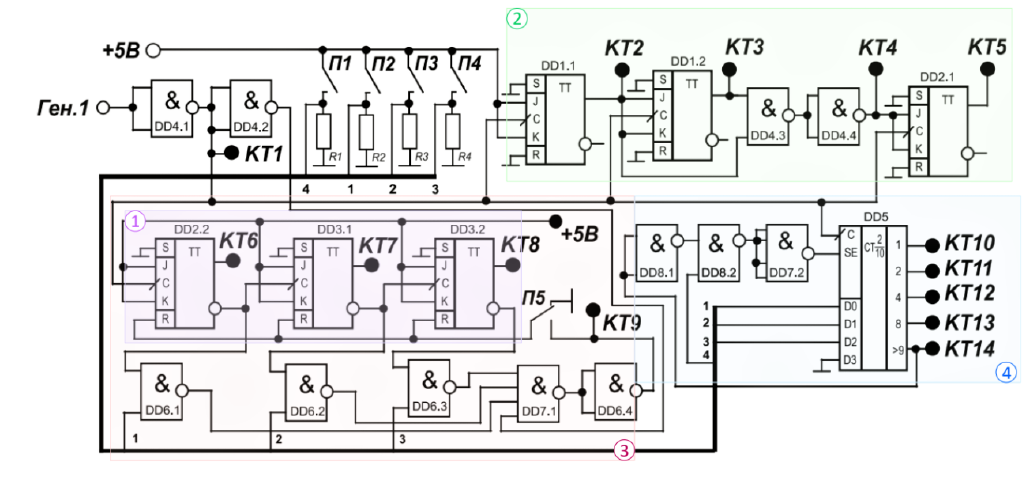
\includegraphics[width=0.7\linewidth]{1.png}}
	\caption{Схеми лiчильникiв що дослiджуються в цiй лабораторнiй роботi.}
	\label{ris1}
\end{figure}



\begin{center}
\textbf{Робоче завдання}
\end{center}
1)  Вивчити принцип дiї лiчильникiв за допомогою лекцiйного матерiалу та пiд-
ручникiв.\\
 
2) Накреслити часовi дiаграми роботи лiчильникiв, якi можна очiкувати зва-
жаючи на теоретичнi вiдомостi для:\\
2.1) лiчильника послiдовного типу (що ми очiкуємо побачити на виводах
КТ1, КТ6 - КТ8)\\
2.2) лiчильника паралельного типу (що ми очiкуємо побачити на виводах
КТ1 - КТ5)\\
2.3) двiйково-десяткового лiчильника (що ми очiкуємо побачити на виводах
КТ1, КТ10 - КТ14)\\
2.4) лiчильника з довiльним коефiцiєнтом перерахунку (що ми очiкуємо по-
бачити на виводах КТ1, КТ6 - КТ9).

\begin{center}
\textbf{Результати вимiрювань}
\end{center}

\begin{figure}[h!]
	\center{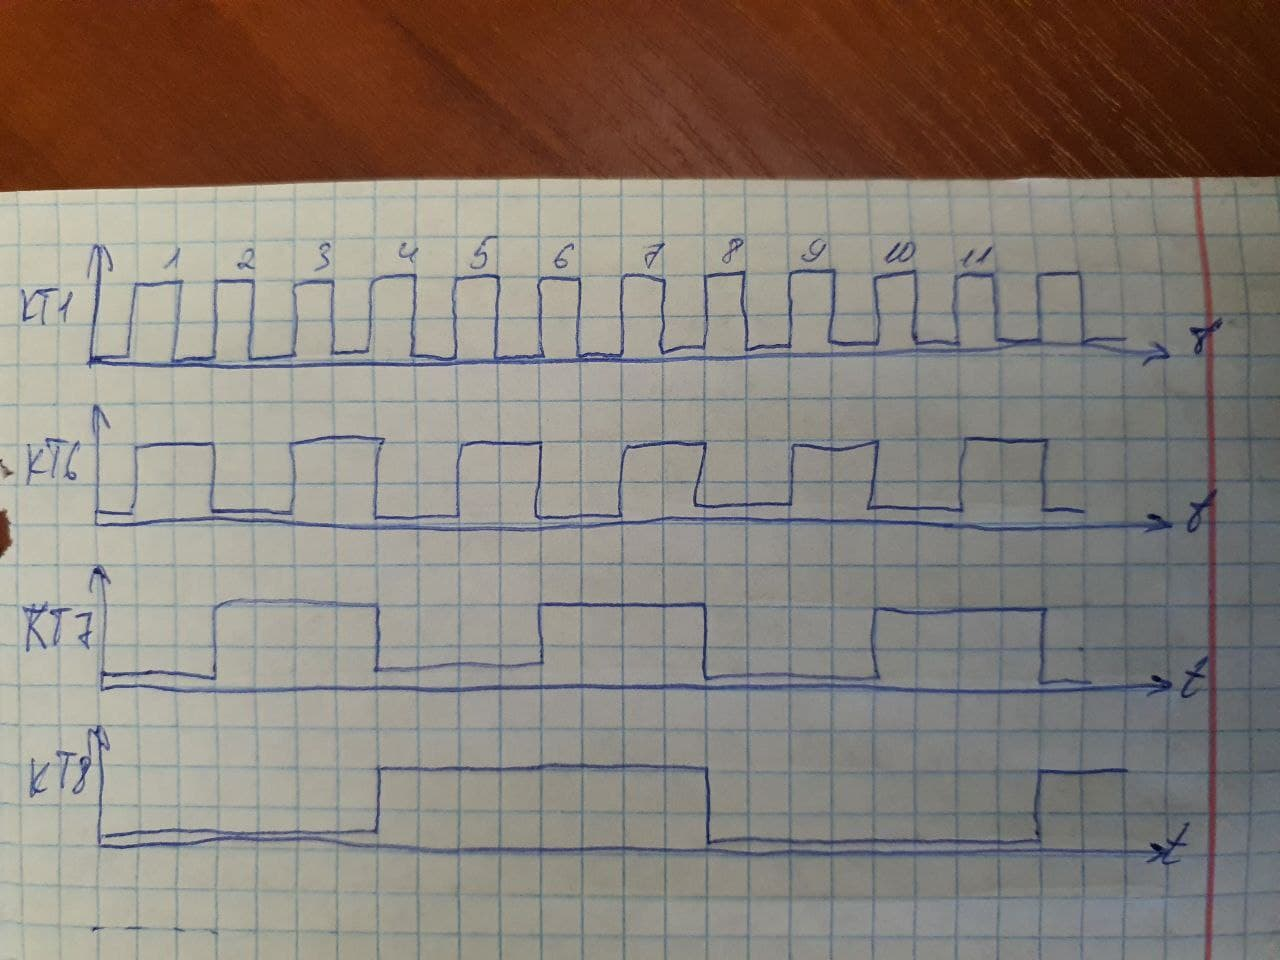
\includegraphics[width=0.8\linewidth ]{1.jpg}}	
	\caption{Часовi дiаграми двiйкового лiчильника послiдовного типу.} 
\end{figure}
 
\begin{figure}[h!]
	\center{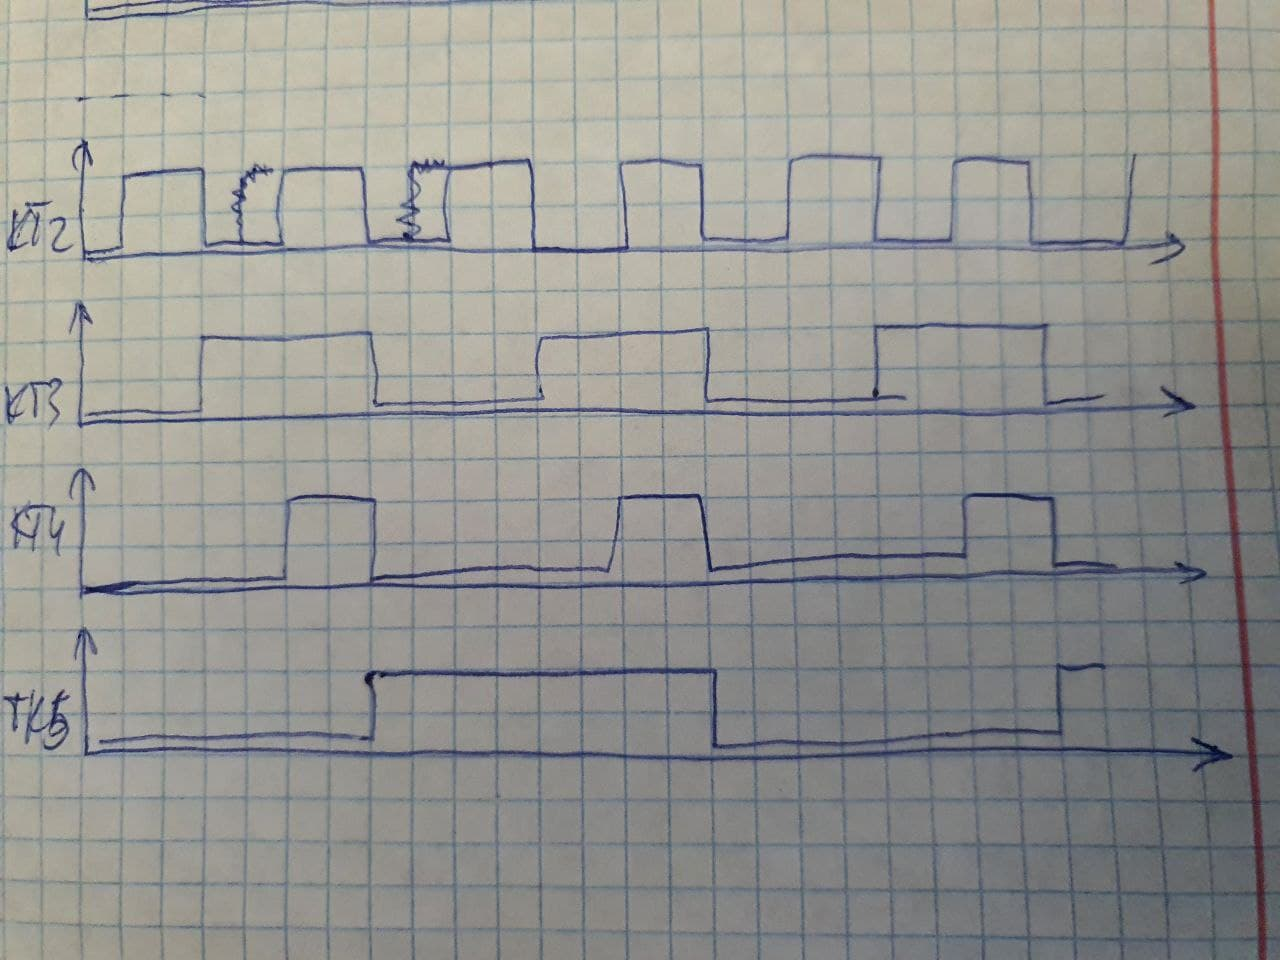
\includegraphics[width=0.8\linewidth ]{2.jpg}}	
	\caption{Часовi дiаграми двiйкового лiчильника паралельного типу.} 
\end{figure}

\begin{figure}[h!]
	\center{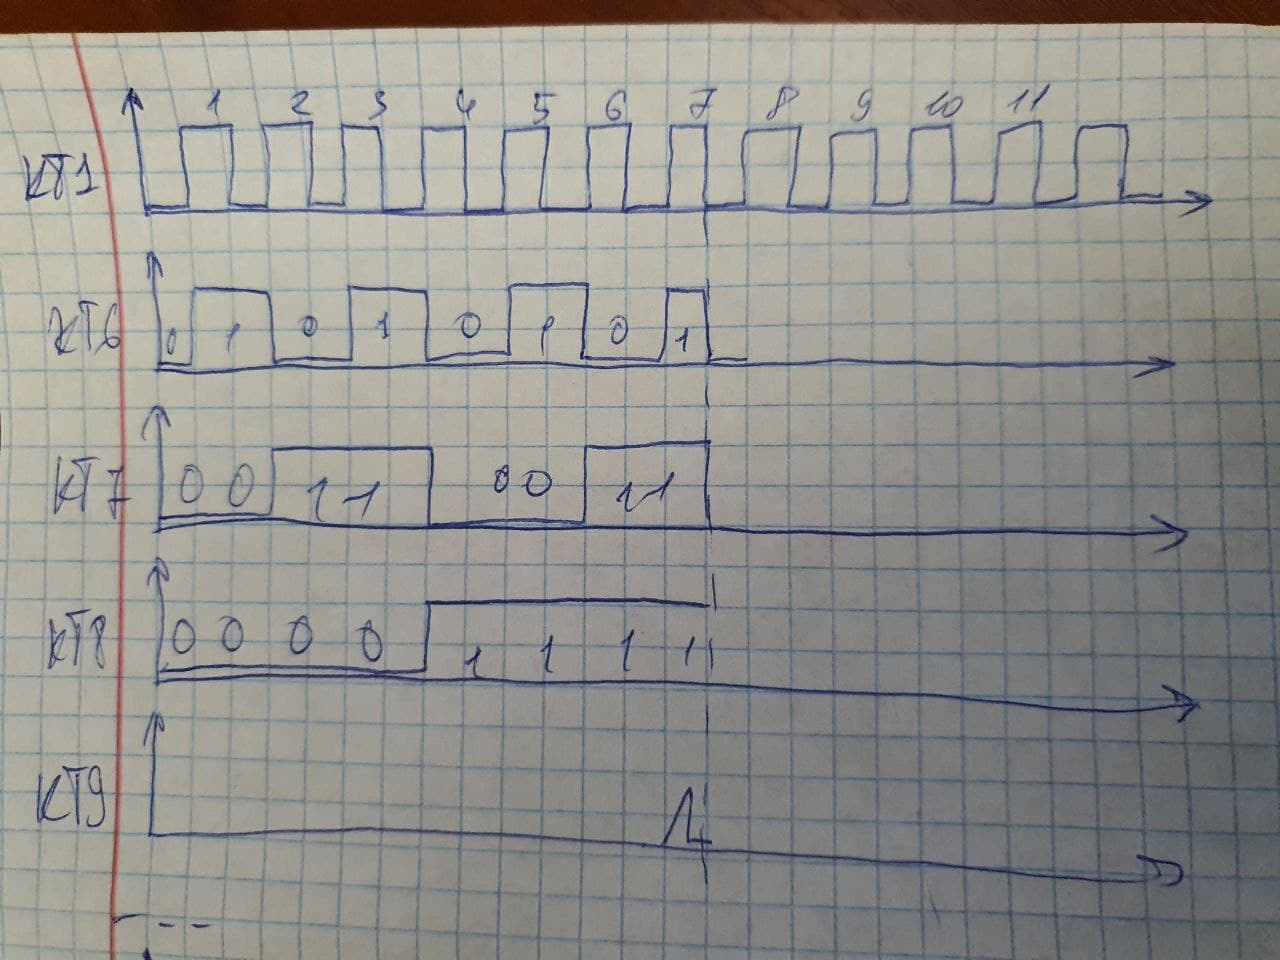
\includegraphics[width=0.8\linewidth ]{3.jpg}}	 
	\caption{ Часовi дiаграми лiчильника з довiльним коефiцiєнтом перерахунку.}
\end{figure}

\begin{figure}[h!]
	\center{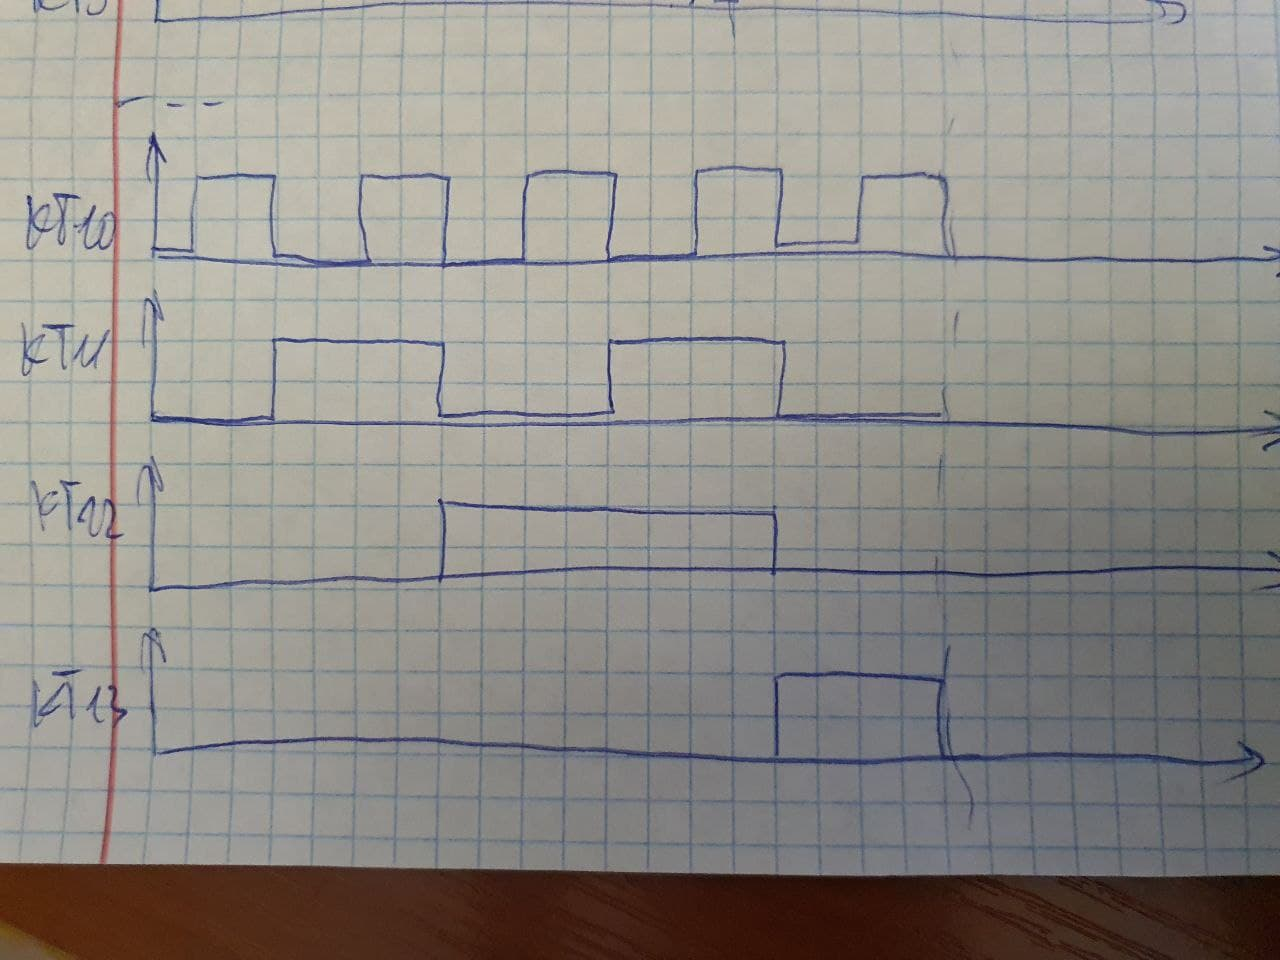
\includegraphics[width=0.8\linewidth ]{4.jpg}}	
	\caption{Часовi дiаграми двiйково - десяткового лiчильника (N = 0).} 
\end{figure}

\begin{figure}[h!]
	\center{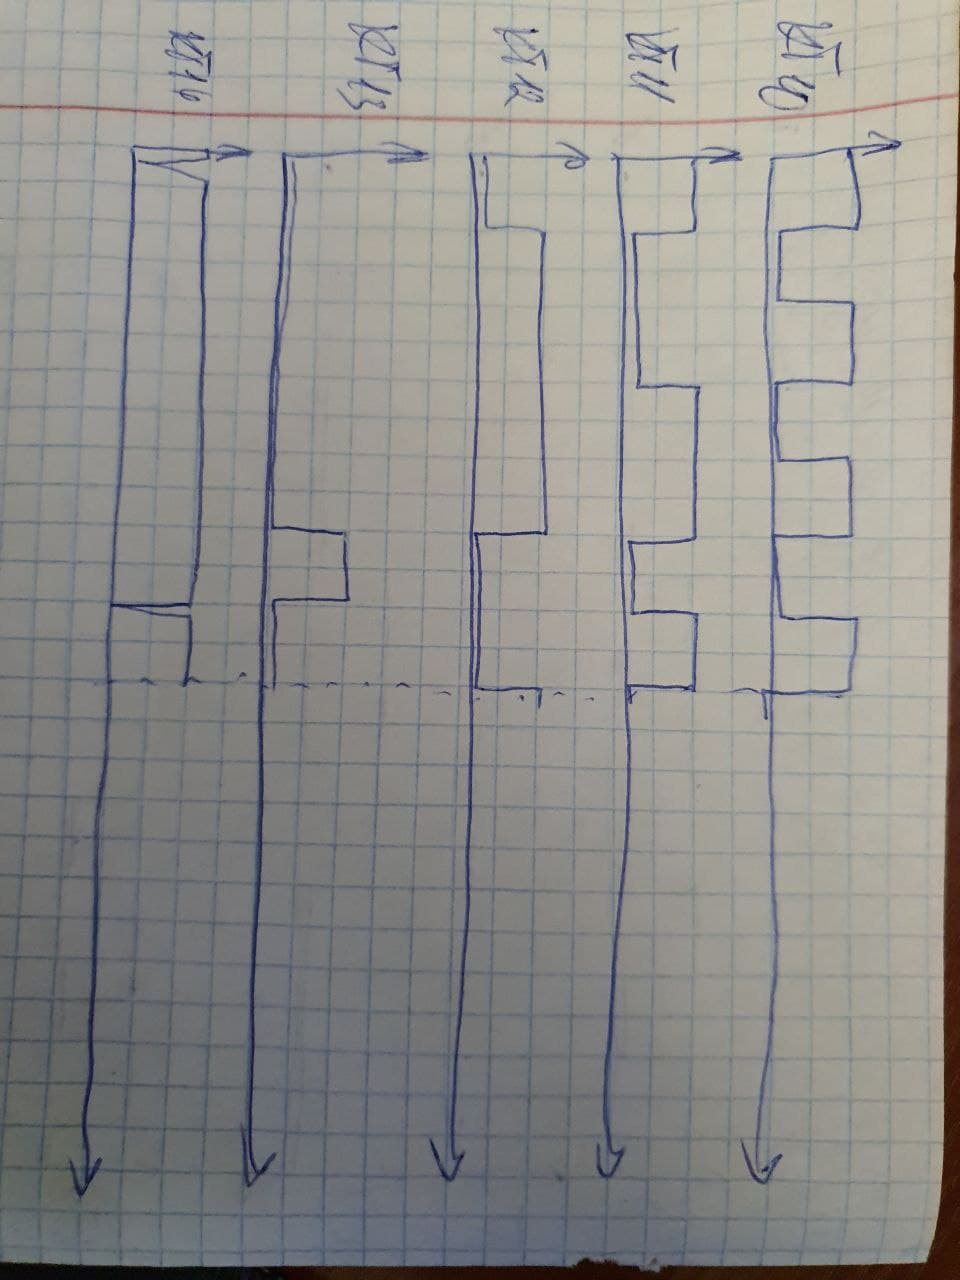
\includegraphics[width=0.8\linewidth, angle=90]{5.jpg}}	
	\caption{Часовi дiаграми двiйково - десяткового лiчильника (N = 3).} 
\end{figure}


\begin{figure}[h]
	\center{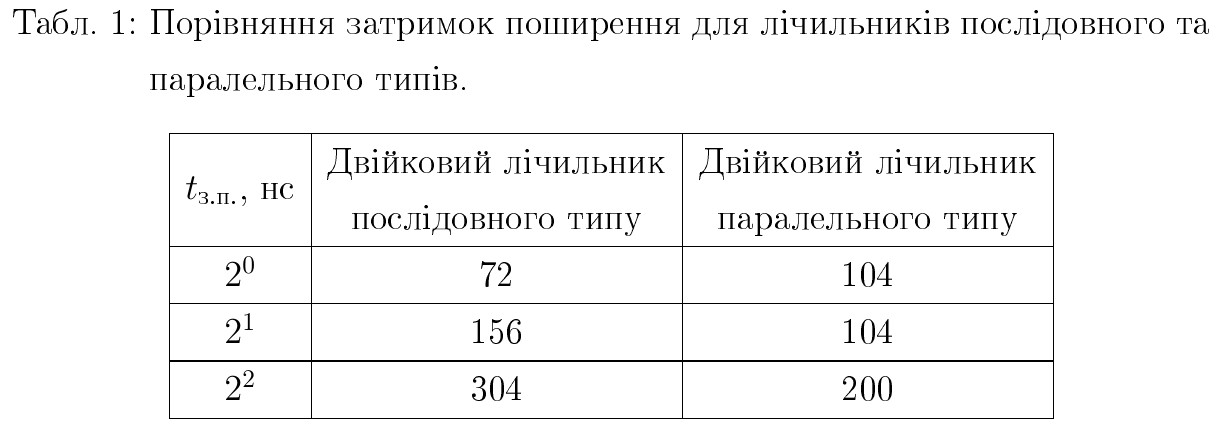
\includegraphics[width=0.8\linewidth]{2.png}}
 
\end{figure}

\clearpage 
\newpage
\begin{center}
\textbf{\fbox{Висновок}}
\end{center}
 В ході лабораторної роботи було досліджено різні лічильники, такі як: Двійковий лічильник (послідовного та паралельного типу), з довільним коефіцієнтом перерахунку та з режимом завантаження константи, та їх принципи роботи, відліку та перенесення лічення на перший розряд.
У двiйковому лiчильнику з послiдовним переносом перемикання старших розрядiв вiдбувається чiтко коли перемкнуться молодшi
розряди, саме це i є лiчильник з послiдовним переносом. Такi схеми простi,
але як ми бачимо з таблицi 1, подальше збiльшення кiлькостi тригерiв веде
до збiльшення затримки поширення в два рази за кожний тригер. У двiйковому з паралельним переносом точка КТ4 - вона є коректуючою для розряду КТ5 у тому планi, що на-
вiть якщо молодший розряд КТ3 перемкнеться трошки пiзнiше - все одно
при переходi КТ4 в 0 КТ5 чiтко перемкнеться також в 0. В цьому випад-
ку затримка перемикання розряду КТ5 визначатиметься затримкою лише
пари вентилiв Шефера, але ж це набагато краще нiж затримка через цiлий
тригер.

\clearpage 
\newpage
\begin{center}
\textbf{\fbox{Захист}}
\end{center}
 \begin{figure}[h!]
	\center{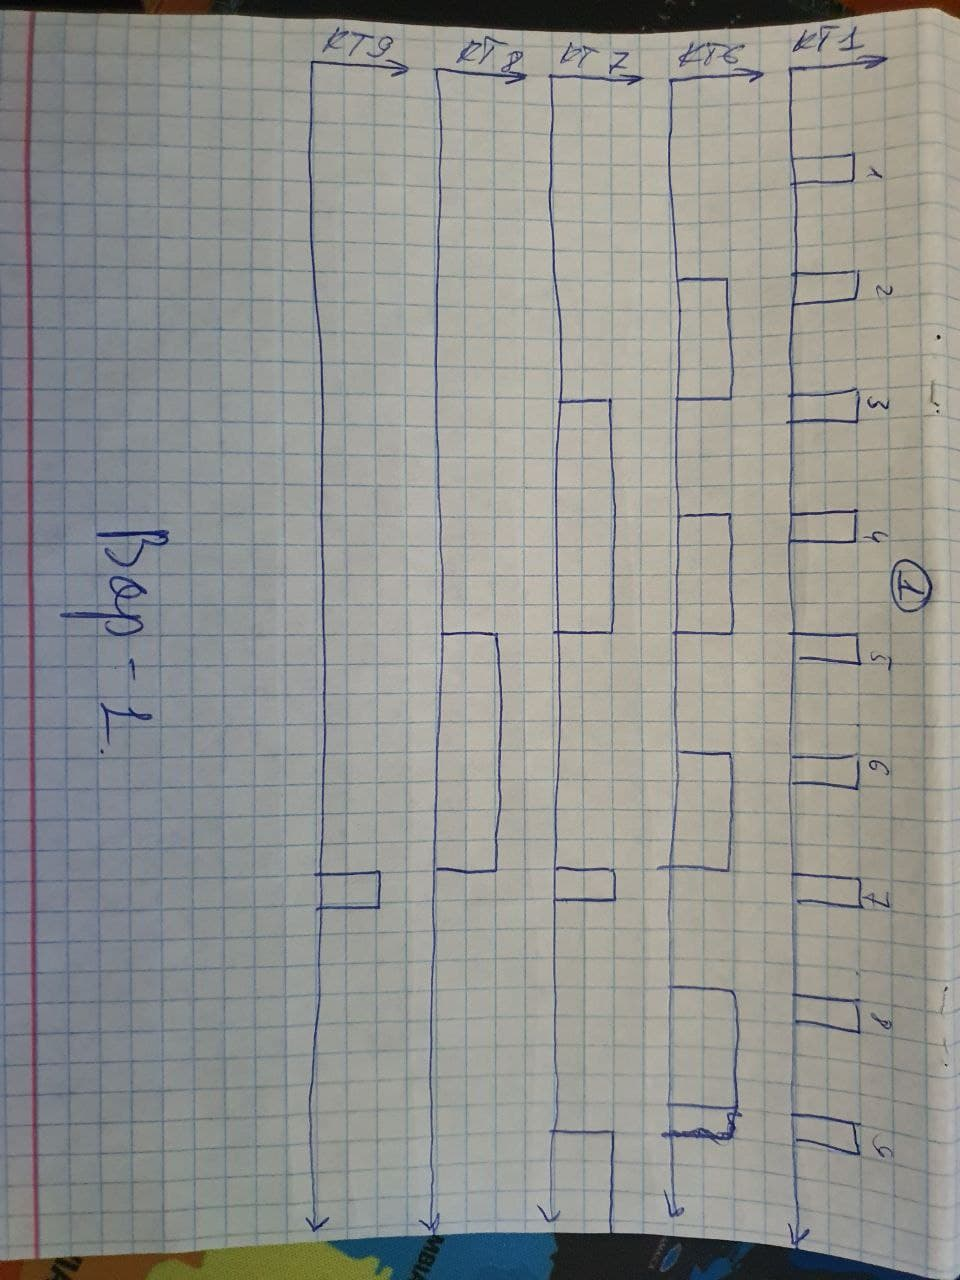
\includegraphics[width=0.8\linewidth, angle=90]{6.jpg}}	
	 
\end{figure}

\begin{figure}[h!]
	\center{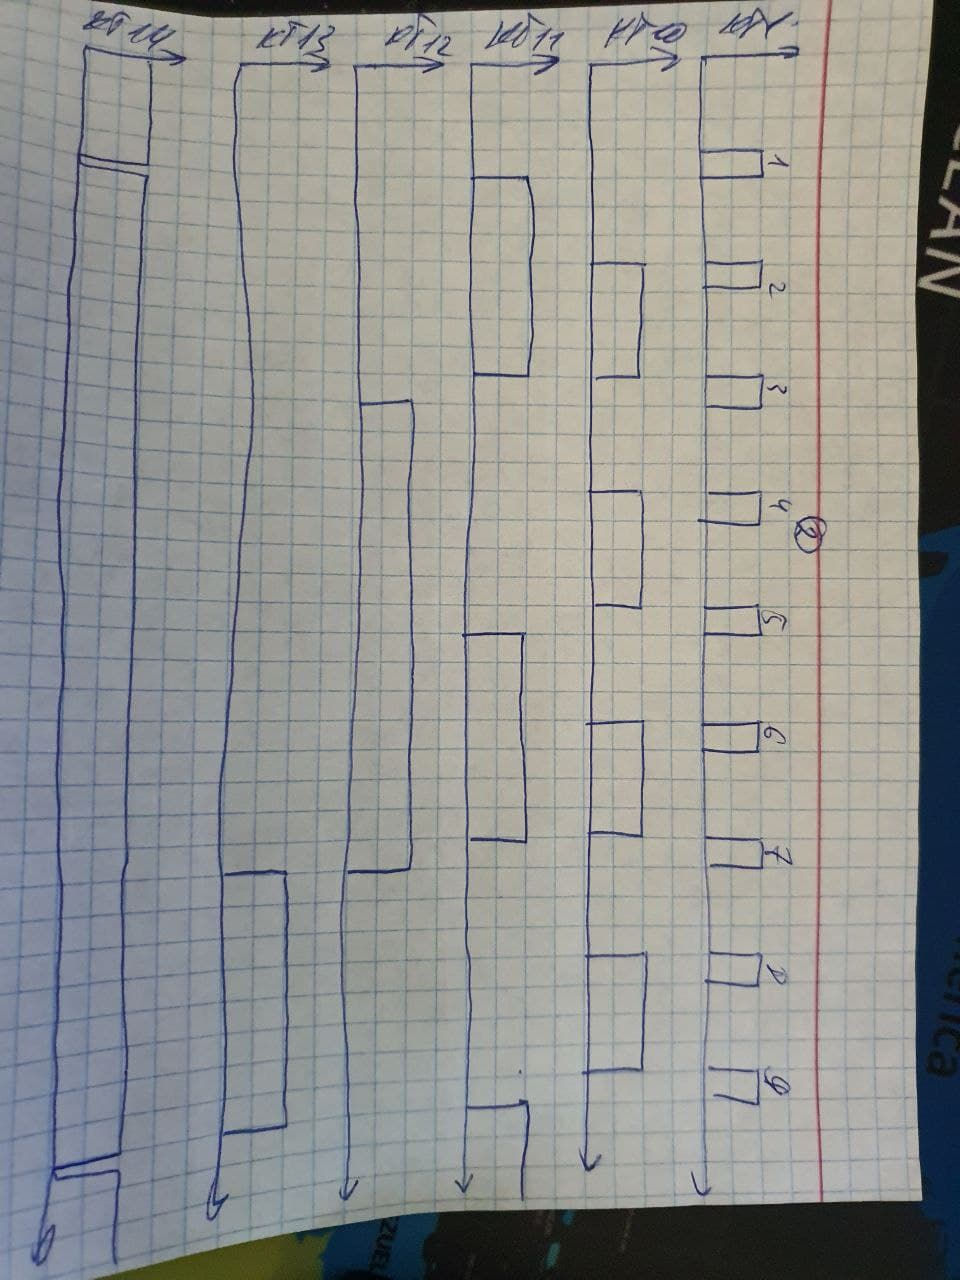
\includegraphics[width=0.8\linewidth, angle=90]{7.jpg}}	
	 
\end{figure}
 




\end{document}